% !TEX root = ../../../main.tex
% 来源：高中物理甲种本·第三册（电磁·光学·近代物理）
% 章节：交流电 / 感应电动机
% 原始文件：3.tex，行 1875-1890
% 类型：tikz
% ---
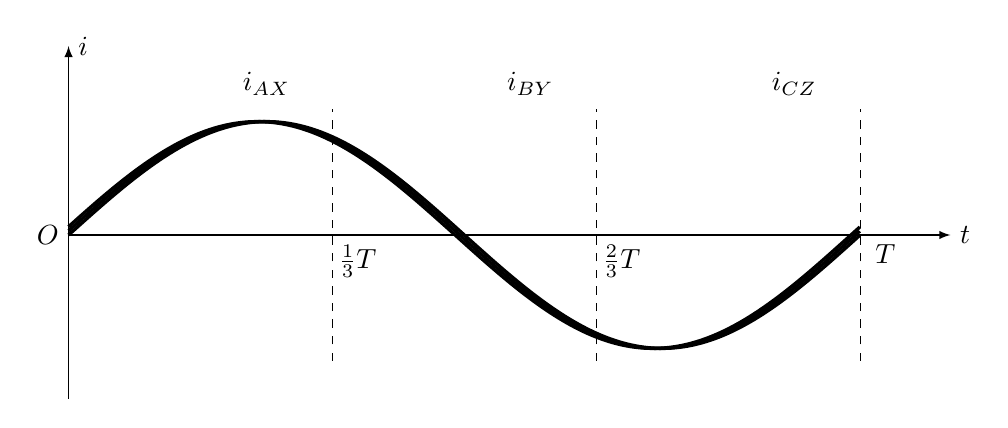
\begin{tikzpicture}[>=latex, scale=1.6]
    \draw[->] (0,-1.3)--(0,1.5)node [right]{$i$};
    \draw [->](0,0)node[left]{$O$}--(7,0)node [right]{$t$};
    \draw [very thick] plot [domain=0:3.1416*2, samples=1000, variable=\x] (\x, {0.9*sin(\x r)}) ;
    \draw [very thick] plot [domain=0:3.1416*2, samples=1000, variable=\x] (\x, {0.9*sin(3.1416*2/3+\x r)}) ;
    \draw [very thick] plot [domain=0:3.1416*2, samples=1000, variable=\x] (\x, {0.9*sin(3.1416*4/3+\x r)}) ;
    \node at (3.1416/2, 1.2){$i_{AX}$};
    \node at (3.1416/2+3.1416*2/3, 1.2){$i_{BY}$};
    \node at (3.1416/2+3.1416*4/3, 1.2){$i_{CZ}$};
\draw[dashed] (3.1416*2/3, -1)--(3.1416*2/3, 1);
\draw[dashed] (3.1416*4/3, -1)--(3.1416*4/3, 1);
\draw[dashed] (3.1416*6/3, -1)--(3.1416*6/3, 1);
\node at  (3.1416*2/3+.2, 0)[below]{$\frac{1}{3}T$};
\node at  (3.1416*4/3+.2, 0)[below]{$\frac{2}{3}T$};
\node at (3.1416*6/3+.2, 0)[below]{$T$};
    \end{tikzpicture}
